\chapter{Tokamak Physics}
In this chapter, all units are SI with the exception of temperature,
which is defined in the historical units of eV (electron-volts).\\

\noindent
$e$ is the fundamental charge unit\\
$Z$ is the number of nuclear protons\\
$R_0$ is the major radius of a toroidal plasma\\
$a$ and $b$ are the horizontal and vertical minor radii of a toroidal plasma\\
\indent Note: $a=b$ for circular cross sections, and $a$ is used by convention\\
$R$ and $r$ denote lengths in the major and minor radii, respectively\\
$\theta$ and $\phi$ are the poloidal and toroidal angular coordinates, respectively\\
$B_x$ is the magnetic field in direction $x$\\
$B_{xa}$ is the magnetic field evaluated at the plasma edge in direction $x$\\
$I_p$ is the toroidal plasma current\\
$p$ is the plasma pressure\\
$v$ is velocity of the plasma\\

\section{Fundamental Definitions}

\index{$\epsilon$}
\index{Inverse aspect ratio}
\noindent
Inverse aspect ratio \scite{wesson}{117}
\fla{ \epsilon &= \frac{a}{R_0} &}

\index{Elongation}
\noindent
Plasma elongation \scite{wesson}{741}
\fla{\kappa &= \frac{b}{a} &}

\index{triangularity}
\noindent
Plasma triangularity \scite{wesson}{741}
\fla{\delta &= \frac{(c+d)/2}{a} &}
\indent where c, d are distances to the top of the plasma and the x-point, \\
\indent respectively, from the plasma center.\\

\index{Large aspect ratio expansion}
\noindent
Large aspect ratio expansion ($\epsilon \ll 1$) \scite{freidberg-PP}{280}
\fla{ \frac{1}{R} &\approx \frac{1}{R_0}\left(1-\frac{r}{R_0}\cos\theta\right) &}

\index{Surface area of a torus}
\noindent
Surface area of a torus 
\fla{ S_\mathrm{c-torus} &= 4\pi^2aR_0 &\hspace{0.5cm} \text{(Circular cross section) \scite{jeffrey}{24}}\\
      S_\mathrm{e-torus} &= 8\pi aR_0E(k) \approx 4\pi^2aR_0\left(\frac{1+\kappa^2}{2}\right)^{1/2} & \hspace{0.5cm} \text{(Elliptical cross section) \cite{wolfram}}}
\noindent

\index{Volume of a torus}
\noindent
Volume of a torus 
\fla{ V_\mathrm{c-torus} &= 2\pi^2a^2R_0 & \hspace{0.5cm} \text{(Circular cross section) \scite{jeffrey}{24}}\\
      V_\mathrm{e-torus} &= 2\pi^2a^2\kappa R_0 & \hspace{0.5cm} \text{(Elliptical cross section)} \cite{wolfram}}

\index{Toroidal plasma volume}
\noindent MHD toroidal plasma volume \scite{freidberg-MHD}{112}
\fla{V(\psi) &= \int\limits_{0}^{2 \pi} \! \int\limits_{0}^{2 \pi} \! \int\limits_{0}^{\hat{r}} \! R r dr d\theta d\phi & \\
 &= \pi R_{0} \int\limits_{0}^{2 \pi} \! d \theta \hat{r}^{2} \left[ 1 + \frac{2}{3} \left( \frac{\hat{r}}{R_{0}} \right) \cos \theta \right] \hspace{0.5cm} \text{ (low aspect ratio)}&}


\index{Plasma pressure}
\noindent
Volume averaged plasma pressure~~\cite{authors}
\fla{ \langle p \rangle &= \frac{1}{V}\!\!\!\!\int\limits_{volume}\!\!\!\! p\,d\tau &}

\index{Toroidal beta}
\noindent
Toroidal plasma beta \scite{freidberg-MHD}{71}
\fla{ \beta_t &= \frac{2\mu_0\langle p \rangle}{B_{\phi a}^2} &}

\index{Poloidal beta}
\noindent
Poloidal plasma beta \scite{freidberg-MHD}{71}
\fla{ \beta_p &= \frac{2\mu_0\langle p \rangle}{B_{\theta a}^2} = \frac{8\pi^2a^2 \kappa^{2}\langle p \rangle}{\mu_0 I_p^2} &}

\index{Radial electric field}
\noindent Radial electric field in a rotating toroidal plasma~~\cite{authors}
\fla{\textrm{E}_{r} &\approx \textrm{v}_{\phi} \textrm{B}_{\theta} - \textrm{v}_{\theta} \textrm{B}_{\phi} +\frac{1}{Z_{i} e n} \nabla p & }


%\subsection{Definitions of Plasma Beta in Pinches}
%\begin{table}[h!]
%  \begin{tabular}{l l}
%    \hline
%    Name & $\beta$\\
%    \hline\hline
%    $\theta$ pinch & $2 \mu_{0} <p>/B_{za}^{2}$\\
%    z pinch & $2 \mu_{0} <p>/B_{\theta a}^{2}$\\
%    Screw Pinch & $2 \mu_{0} <p>/\left( B_{za}^{2}+B_{\theta a}^{2} \right)$
%  \end{tabular}
%\end{table}

\section{Magnetic Topology}

\index{Toroidal magnetic field}
\noindent
Toroidal magnetic field for plasma confinement~~\cite{authors}
\fla{ B_\phi &\approx \frac{B_\phi(r)R_0}{R} &\\
  &\approx \frac{B_\phi(r)}{1-\epsilon\cos\theta} \text{  (valid for $\epsilon \ll 1$)} &}

\index{Poloidal magnetic field}
\noindent
Poloidal magnetic field for plasma confinement~~\cite{authors}
\fla{ B_\theta &\approx \frac{\mu_0 I_p(r)}{2\pi r} &}

\index{Safety factor}
\noindent
Safety factor (general) \scite{wesson}{111}
\fla{ q(r) &= \frac{\text{\# of toroidal field line orbits at r}}{\text{\# of poloidal field line orbits at r}} &\\}

\index{$q$, $q_*$}
\noindent
Safety factor for cylindrical plasma $(r,\theta,z)$ \scite{wesson}{112}
\fla{ q(r)_{\mathrm{cyl}}  &= \frac{rB_\phi(r)}{RB_\theta(r)} = \frac{2\pi r^2 B_\phi(r)}{\mu_0 I_p(r) R} &}

\noindent
Safety factor for toroidal plasma $(R,\theta,\phi)$ \scite{freidberg-PP}{288}
\fla{ q(r^*)_{\mathrm{tor}} &= \frac{1}{2\pi} \int\limits_0^{2\pi}\frac{rB_\phi}{RB_\theta}\,d\theta &\\
  &= \frac{r_0 B_\phi(r_0)}{R_0 B_\theta(r_0) \left(1 - r_0^2/R_0^2\right)^{1/2}} &}
\indent where the flux surfaces $r^*=r_0$ are circles.\\

\noindent
Safety factor at the edge for toroidal plasma $(R,\theta,\phi)$ \scite{freidberg-PP}{387}
\fla{ q_* &\equiv \frac{2\pi a^2 B_0}{\mu_0 R_0 I_{p}} = \frac{\pi k}{4 E(k) (\beta / \epsilon)^{1/2}} &}
\hangindent=0.25in where $E(k)\approx \left[ k^{2}+\pi^{2}/4(1-k^{2})\right]$ is the complete elliptic integral of the second kind and the definition of $k$ is given by
\fla{\frac{B_i^{2}}{B_{0}^{2}} & \equiv 1-\frac{2\mu_{0}p}{B_{0}^{2}} + \frac{4 \epsilon \mu_{0}p}{k^{2}B_{0}^{2}}\left( 2-k^{2} \right) &}

\noindent
Approximate edge safety factor for a large aspect ratio toroidal plasma \scite{freidberg-PP}{414}
\fla{q_{*} &\approx \frac{2 \pi B_{0}a^{2}}{\mu_{0}R_{0}I_{p}} \left( \frac{1+\kappa^{2}}{2}\right) &} %Freidberg 13.171

\index{Magnetic shear}
\noindent
Magnetic shear \scite{freidberg-PP}{408}
\fla{s &= \frac{r}{q}\frac{dq}{dr} &}


\section{Magnetic Inductance}

\index{Magnetic inductance}
\noindent
Definition of magnetic inductance \scite{freidberg-PP}{281}
\fla{ \frac{1}{2}LI^2 \, &\equiv \!\!\! \int \limits_\mathrm{volume} \!\!\! \frac{B^2}{2\mu_0}\,d\tau &}

\noindent
Normalized inductance per unit length [dimensionless] \scite{freidberg-PP}{281}
\fla{ \ell &\equiv \frac{L/2\pi R_0}{\mu_0/4\pi} = \frac{2L}{\mu_0 R_0} &}

\index{Inductance of plasma}

\index{Internal inductance}
\noindent
Internal inductance of a toroidal plasma \scite{freidberg-PP}{281}
\fla{ L_i &= \frac{8\pi R_{0}}{I_p^2} \int\limits_0^a \frac{B_\theta^2}{2\mu_0}\,r dr = \frac{\mu_0 R_0 \langle B_\theta^2 \rangle}{2B_{\theta a}^2} &\\
  \ell_i &= \frac{\langle B_\theta^2\rangle}{B_\theta^2(a)} &}

\index{External inductance}
\noindent
External inductance of a toroidal plasma \scite{freidberg-PP}{281}
\fla{ L_e &= \frac{8 \pi R_{0}}{I_p^2} \int\limits_a^\infty \frac{B_\theta^2}{2\mu_0}\,r dr = \mu_0 R_0\left(\ln \frac{8R_{0}}{a} - 2\right) &\\
  \ell_e &= 2\ln\frac{8R_{0}}{a} - 4 &}


\index{Toroidal force balance}
\section{Toroidal Force Balance}
\noindent
Equation of toroidal force balance \scite{freidberg-PP}{279}
\fla{ &\int \mathbf{\hat{R}} \cdot \left(\mathbf{J} \times \mathbf{B} - \nabla p\right)\,d\tau = 0 &}
\indent where
\fla{ \mu_0 \mathbf{J} &= \nabla \times \mathbf{B} = \frac{R_0}{R}\frac{\partial B_\phi}{\partial r}\mathbf{\hat{\boldsymbol{\theta}}} - \frac{1}{r}\frac{\partial}{\partial r}\left(\frac{R_0}{R}rB_\theta\right)\mathbf{\hat{\boldsymbol{\phi}}} &}
\fla{&\mathbf{\hat{R}} \cdot \mathbf{J} \times \mathbf{B} =& \\
  & -\cos\theta \left[\frac{R_0^2}{R^2}\frac{\partial}{\partial r}\left(\frac{B_\phi^2}{2\mu_0}\right)+\frac{R_0 B_\theta}{\mu_0 r R}\frac{\partial}{\partial r}\left(\frac{R_0}{R}rB_\theta\right)\right]-\frac{B_\mathrm{vert}}{\mu_0 r}\frac{\partial}{\partial r}\left(\frac{R_0}{R}rB_\theta\right) &}

\index{Hoop force}
\noindent
The hoop force\scite{freidberg-PP}{280}
\fla{ \mathbf{F_\mathrm{hoop}} &= \frac{I_p^2}{2}\frac{\partial}{\partial R}\left(L_i + L_e\right)\,\mathbf{\hat{R}} 
  = 2\pi^2a^2(\ell_i + \ell_e + 2)\frac{B_{\theta a}^2}{2\mu_0} \,\mathbf{\hat{R}} &\\
  &= \frac{\mu_0 I_p^{2}}{2}\left(\ln \frac{8R}{a} - 1 + \frac{\ell_i}{2}\right) \, \mathbf{\hat{R}}}

\index{Tire tube force}
\noindent
The tire tube force \scite{freidberg-PP}{280}
\fla{ \mathbf{F_\mathrm{tire}} &= 2\pi^2a^2\langle p \rangle \,\mathbf{\hat{R}} &\\
  &= \frac{\mu_0 I_p^2\beta_p}{4}\,\mathbf{\hat{R}}&}
%\indent where $\beta_p = (8\pi^2a^2\langle p \rangle)/(\mu_0 I_p^2)$ has been used.\\

\index{1/R force}
\noindent
The 1/R force \scite{freidberg-PP}{280}
\fla{ \mathbf{F_\mathrm{1/R}} &= 2\pi^2a^2\left(\frac{B_{\phi a}^2}{2\mu_0} - \frac{\langle B_\phi^2\rangle}{2\mu_0}\right) \,\mathbf{\hat{R}} &\\
  &= \frac{\mu_0 I_p^2}{4}\left(\beta_p -1\right)\,\mathbf{\hat{R}} &}
\indent where $\langle p \rangle = \frac{1}{2\mu_0}\left(B_{\phi a}^2 - \langle B_\phi^2 \rangle + B_{\theta a}^2\right)$\\
\indent have been used.\\

\noindent
The vertical field force on toroidal plasma ring \scite{freidberg-PP}{282}
\fla{ \mathbf{F_\mathrm{vert}} &= -2\pi R_0 B_\mathrm{vert}I_p \,\mathbf{\hat{R}}&}

\index{Vertical magnetic field}
\noindent
The vertical magnetic field required to balance toroidal forces \scite{freidberg-PP}{282}
\fla{ B_\mathrm{vert} &= \frac{\mathbf{F_\mathrm{hoop}}+\mathbf{F_\mathrm{tire}}+\mathbf{F_\mathrm{1/R}}}{2\pi R_0 I_p} &\\
  &= \frac{\epsilon}{4}B_{\theta a}\left(\ell_e + \ell_i + 2 + \frac{2\mu_0\langle p \rangle}{B_{\phi a}^2} + \frac{B_{\phi a}^2-\langle B_\phi^2\rangle}{B_{\theta a}^2}\right) &\\
  &= \frac{\mu_0 I_p}{4\pi R_0}\left(\ln\frac{8R}{a} - \frac{3}{2} + \frac{\ell_i}{2} + \beta_p\right) &}
\index{Shafranov shift}
Shafranov shift of the plasma center \scite{freidberg-MHD}{2129}

\fla{ \Delta &= \frac{b^2}{2 R_{0}} \left[ \left( \beta_{p} + \frac{l_{i} -1 }{2} \right) \left( 1 -\frac{a^{2}}{b^{2}} \right) + \ln \frac{b}{a} \right] - \frac{B_{vert}}{B_{\theta1}(b)}&}

\index{Paramagnetic plasmas}
\index{Diamagnetic plasmas}
\section{Plasma Para- and Dia-Magnetism}
Global pressure balance equation in a screw pinch  \scite{freidberg-PP}{270}
\fla{\langle p\rangle &= \frac{1}{2 \mu_{0}} \left( B_{za}^{2} - \langle B_{z}^{2} \rangle + B_{\theta a}^{2} \right) &}
\indent can be rearranged to give
\fla{\beta_{p} &= \frac{B_{za}^{2}-\langle B_{z}^{2} \rangle}{B_{\theta a}^{2}}+1 &}
\begin{align*}
  \indent 
  \mathrm{Diamagnetic:} & ~~\beta_{p} < 1 & \mathrm{Paramagnetic:} & ~~\beta_{p} > 1
\end{align*}


\section{MHD Stability Limits}
Using experimental data from a wide variety of tokamaks, empirical
scalings for critical tokamak instabilities have been constructed.
Units: current in MA, length in m, magnetic field in T, and density in
$n_{20} = n/10^{20}$.

\index{Troyon limit}
\index{Beta limit|see{Troyon limit}}
\begin{enumerate}
\item{Beta limits (no plasma shaping)
  \begin{flalign*}
    \beta_t &\le \beta_L\frac{I}{a B_\phi} & \\
    \beta_L &= 0.028 \text{  Troyon kink limit - no wall \cite{troyonlimit}} & \\
    \beta_L &= 0.044 \text{   Sykes ballooning limit - no wall} & \\
    \beta_L &= 0.06 \text{  kink - ideal conducting wall}  &
  \end{flalign*}
}
%\item{The Troyon (or beta) limit (plasma elongation $\kappa$)
%\fla{ \beta_t &\le 0.15\frac{\kappa \epsilon}{q_j} &}

%\noindent where $\epsilon = \frac{a}{R_0}$ and $q_j \approx 2\pi a^2 \kappa B_\phi/I_p R_0$
%}
\index{$\beta_{N}$}
\item{Definition of $\beta_{N}$ \scite{wesson}{347}
  \fla{\beta_{N} &\equiv \beta_{t} [\%] \,\frac{aB_{\phi}}{I_p \textrm{[MA]}} &}
}
  
\index{Greenwald limit}
\index{Density limit|see{Greenwald limit}}
\item{The Greenwald (or Density) Limit \scite{wesson}{377}
  \fla{ n_{20} \le n_G &= \frac{I_{p} \textrm{[MA]}}{\pi a^2} &}
}
\end{enumerate}

\section{Tokamak Heating and Current Drive}
\begin{enumerate}
\item{Ohmic plasma heating

\index{Ohmic heating}
The neo-classical resistivity approximation is \scite{freidberg-PP}{538}

\fla{ \eta_{||} &= \frac{1}{\left[1-(r/R_{0})^{1/2}\right]^{2}} \eta_{||}^{\textrm{Spitzer}} &}

\noindent Plugging in for the current as $J_{||}=E_{0}/\eta_{||}$ \scite{freidberg-PP}{539}

\fla{P_{\Omega} &= \left( \frac{5.6 \times 10^{-2}}{ 1-1.31 \epsilon^{1/2} + 0.46 \epsilon} \right) \left( \frac{R_{0} \left( I \textrm{[MA]} \right)^{2}}{a^2 \kappa T_{keV}^{3/2} } \right) \textrm{[MW]} &}
}

\item{Neutral beam plasma heating \scite{wesson}{246-248}

\index{Neutral beam heating}
%Neutral beams deposit their energy via collisions with the ions and electrons in the plasma. The energy deposition from the beam is then calculated to be

\fla{ P &= m_{b} \frac{n e^{4} \textrm{ln} \Lambda}{2 \pi \epsilon_{0}^{2} m_{b}^{2}} \left( \frac{2 m_{e}^{1/2} E_{b}}{ 3 (2 \pi)^{1/2} T_{e}^{3/2}} + \frac{m_{b}^{3/2}}{2^{3/2} m_{i} E_{b}^{1/2}} \right) &}

\indent where $E_{b}$ is the energy of the beam.

\noindent The critical beam energy when the ions and the electrons are heated equally by the beam is

\fla{E_{c} &= 14.8 \frac{A_{b}}{A_{i}^{2/3}} T_{e} &}
}
\end{enumerate}
\subsection{Current Drive}

\begin{enumerate}

\item{Inductive current

\index{Inductive current}
This current is driven via the central solenoid. The current distribution is 
calculated through the use of Faraday's law and $J_{||}=E_{0}/\eta_{||}$. 
Total current normally has to be measured in order to normalize the distrubition of
 current density.
}
\item{Bootstrap current

\index{Bootstrap current}
Bootstrap current is the self-generated current drive in the plasma from trapped and passing electrons in the plasma. 

The exact form of the bootstrap current density is given by \scite{freidberg-PP}{496}

\fla{j_{B} &= -4.71 q \left( \frac{R_{0}}{r} \right)^{1/2} \frac{T}{B_{0}} \left[ \frac{\partial n}{\partial r} +0.04 \frac{n}{T} \frac{\partial T}{\partial r} \right] &}

\noindent The total bootstrap fraction is given by \scite{freidberg-PP}{496}

\fla{f_{B} &\approx -1.18 \frac{\partial}{\partial r}(\textrm{ln} n + 0.04 \textrm{ln} T) / \frac{\partial}{\partial r}(\textrm{ln} r B_{\theta}) \left( \frac{r}{R_{0}} \right)^{1/2}\beta_{p} \sim \epsilon^{1/2} \beta_{p} &}
}
\item{Neutral beam current drive

\index{Neutral beam current drive}
By positioning a neutral beam in the tangential direction, it is
possible to drive both rotation and current. Neutral beam current
drive efficiency scales as (at $E_{b}=40 A_{b} T_{e}$) \cite{cordey}

\fla{I[\mathrm{A}]/P[\mathrm{W}] &\approx \frac{0.06 T_{e}}{n_{20} R Z_{b}}(1-Z_{b}/Z_{\mathrm{eff}}) &}
}

\item{Lower hybrid current drive

\index{LHCD}
Currently one of the most used current drive mechanisms is the lower
hybrid system. It launches a wave that Landau damps on the fast
electron population and preferentially drives electrons in one
direction. \scite{freidberg-PP}{623}

\fla{I[\mathrm{A}]/P[\mathrm{W}] &= 1.17/\left( n_{||}^{2} R_{0} n_{20} \right) &}

\noindent There exists an accessibility condition for the waves which forces an increase in the launched $n_{||}$ \scite{stix}{100}

\fla{n_{||}^{2} &> \left(S^{1/2} + \left| \frac{D^{2}}{P} \right| ^{1/2} \right)^{2} &}

\indent where S, P, and D are defined in Chapter \ref{chap:plasmawaves}.\\
\noindent Because LHCD relies on Landau damping, there is an additional
constraint on the $n_{||}$: Landau damping dominates at $n_{||}^{c}
\gtrsim 7.0/T_{\mathrm{keV}}^{1/2}$ \cite{granatstein}
}

\item{Fast Magnetosonic wave current drive
\index{Fast Magnetosonic wave CD}

Allows peaked on-axis profiles and has the following current drive efficiency \cite{cordey}

\fla{I[\mathrm{A}]/P[\mathrm{W}] &= 0.025 \frac{T_{\mathrm{keV}}}{n_{20} R_{0}} &}
}

\end{enumerate}

\section{Empirical Scaling Laws}

\subsection{Energy Confinement Time Scalings}

\index{Goldston scaling|see{Energy confinement scalings}}
\noindent
Goldston auxiliary heated tokamak scaling (l refers to the plasma size $\sim a$) \scite{wesson}{152}
\fla{\tau_{E} & \sim B_{p}^{2} l^{1.8}/ n T &}

\index{Energy confinement scalings}

\noindent
The ITER-89 L-Mode (ITER89-P) \scite{wesson}{740}
\fla{\tau_E &= 0.048 I_M^{0.85}R_0^{1.2}a^{0.3}\kappa^{0.5}\bar{n}_{20}^{0.1}B_0^{0.2}A^{0.5}P_M^{-0.5} \hspace{0.5cm}\mathrm{[s]} &}

\noindent % Ref:  ITER Physics Basis 1999 (pg 2206, Ch 2, eqn 24)
The ITER-98 L-Mode \cite{iter}
\fla{\tau_E &= 0.023 I_M^{0.96}B_{T}^{0.03}n_{19}^{0.40}M^{0.20}R^{1.83}\epsilon^{-0.06}\kappa^{0.64}P_{MW}^{-0.73} \hspace{0.5cm}\mathrm{[s]} &}

\noindent % Ref:  ITER Physics Basis 1999 (pg 2204, Ch 2, eqn 20)
The ITER-98 (IPB98[y,2]); ELMy H-mode \cite{iter}
\fla{\tau_E &= 0.0562 I_M^{0.93}B_{T}^{0.15}n_{19}^{0.41}M^{0.19}R^{1.97}\epsilon^{0.58}\kappa^{0.78}P_{MW}^{-0.69} \hspace{0.5cm}\mathrm{[s]} &}

\index{Lindear regime scaling}
%\noindent The ITER-98 L-mode confinement only holds above a critical density below which the neo-Alcator scaling is used; 
% this is a weird formula; cited in ITER phys. basis, but came from a Japanese tokamak. Not neo-Alcator.
\noindent Scaling for linear regime energy transport \cite{iter}
\fla{\tau_{E} &= 0.07 n_{20} q \kappa^{0.5}aR^2 \hspace{0.5cm} \text{[s]}&}

\noindent Critical density of linear to saturated regime \cite{iter}
\fla{n_{20} &= 0.65 A_{i}^{0.5}B_{T} q^{-1}R^{-1} &} 

\subsection{Plasma Toroidal Rotation Scaling}

% cite Rice et al.
\index{Rice scaling|see{Toroidal rotation scaling}}
\index{Toroidal rotation scalings}
Plasma toroidal rotation (Rice) scaling \cite{rice}
\fla{\Delta V_{tor} & \propto \Delta W/I_{p} &}

\noindent The 2010 multi-machine scaling database found that (with $v_{a}$ being the Alfv\'en speed) \cite{rice}
\fla{v/v_{a} &= 0.65 \beta_{T}^{1.4} q_{j}^{2.3}&}

\indent where $q_{j} =2 \pi \kappa a^{2} B/\mu_{0} R I_{p}$

\index{L-H mode power scalings}
\subsection{L-H Mode Power Scalings}
\noindent
The ITPA empirical scaling law for the L to H mode transition power threshold \cite{martin} % Y. Martin 2008
%\fla{P_{\text{L-H}} = 2.84 B_t^{0.82}n_e^{0.58}M^{-1}Ra^{0.81} \text{     [MW]} }
\fla{P_{\text{L-H}}\textrm{[MW]} &= 2.15 e^{\pm 0.107} n_{20}^{0.782 \pm 0.037} B_{\text{T}}^{0.772\pm 0.031} a ^{0.975 \pm 0.08} R^{0.999 \pm 0.101} &}

\index{Turbulence}
\section{Turbulence}

Fundamental definitions \scite{wesson}{422-424}
\flatwo{L_{n} &= n/\nabla n & L_{T} = T/\nabla T}{5}
\flatwo{b &= k_{\theta}^2 \rho_{i}^{2} & \eta_{j} = L_{nj}/L_{Tj}}{5}
\fla{\epsilon &= m_{j} v^{2}/2 T_{j} &}

\index{Diamagnetic drift velocity}
\noindent The diamagnetic drift velocity \scite{wesson}{420}
\fla{\textbf{v}_{dj} &= \frac{\textbf{B} \times \nabla p_{j}}{q_{j}n_{j} B^{2}} &}

\index{Diamagnetic drift frequency}
\noindent Diamagnetic frequency \scite{wesson}{421}
\fla{\omega_{*j} &= - \frac{k_{y} T_{j}}{e B n} \frac{dn}{dr} &}

\noindent Ion Larmor radius evaluated at the sound speed \cite{tynan}
\index{$\rho_{S}$}
\fla{\rho_{S} &\equiv c_{s}/\Omega_{i} &}

\noindent Normalized Larmor radius 
\index{$\rho_{*}$}
\fla{\rho_{*} &\equiv \rho_{S}/a &}

\subsection{General Drift Wave Turbulence}

Mixing length estimate \cite{tynan}
\fla{ \tilde{n}^{\textrm{rms}}/n_{0} &\sim 1/k_{\bot} L_{\textrm{n}} &}

\noindent Density fluctuations and plasma potential correlation \cite{tynan}
\fla{ \tilde{n}/n_{0} &\approx \left( e\tilde\phi/kT_{e} \right) \left( 1-i\delta \right)&}

\hangindent=0.25in where $\delta$ is the dissipation of the electron momentum to the background plasma.\\

\noindent Time averaged electrostatic turbulent flux of particles $\tilde{\Gamma}$, momentum $\overleftrightarrow{\mu}$, and heat $\tilde{Q}$ \cite{tynan}

\index{Turbulent flux of particles}
\fla{\tilde{\Gamma} &= - \frac{\langle \tilde{n} \nabla \tilde{\phi} \rangle \times \bar{\textbf{B}}}{\textrm{B}^2} + \langle \tilde{n} \tilde{v}_{||}\rangle \textbf{B}/\textrm{B}&}

\index{Turbulent flux of momentum}
\fla{\overleftrightarrow{\mu} &= \left\langle \left( -\frac{\nabla \tilde{\phi} \times \bar{\textbf{B}}}{\textrm{B}^{2}} + \tilde{v}_{||}\textbf{B}/\textrm{B} \right) \left( -\frac{\nabla \tilde{\phi} \times \textbf{B}}{B^{2}} + \tilde{v}_{||}\textbf{B}/\textrm{B} \right) \right\rangle &}

\index{Turbulent flux of energy}
\fla{\tilde{Q} &\equiv \frac{5}{2} \bar{n}\bar{T} \left[ \frac{1}{\bar{T}} \left( - \frac{\langle \tilde{T}\nabla \tilde{\phi} \rangle \times \bar{\textbf{B}}}{\textrm{B}^2}+ \langle \tilde{T}\tilde{v}_{||} \rangle \textbf{B}/\textrm{B} \right) + \frac{1}{\bar{n}} \left(  - \frac{\langle \tilde{n} \nabla \tilde{\phi} \rangle \times \bar{\textbf{B}}}{\textrm{B}^2} + \langle \tilde{n} \tilde{v}_{||}\rangle \textbf{B}/\textrm{B} \right) \right] &}


\indent where fluctuating values are marked by a tilde and $\langle ~ \rangle$ is a time average. \\

\noindent
Time averaged momentum and and energy fluxes due to fluctuating magnetic fields \cite{tynan}

\index{Magnetic turbulence flux of momentum}
\fla{\overleftrightarrow{\mu}^{EM} & = \frac{\langle \tilde{B}\tilde{B} \rangle}{\mu_{0} \bar{n} M_{i}} &}

\index{Magnetic turbulence flux of energy}
\fla{\tilde{Q}^{EM} &= \frac{\langle \tilde{q}_{||e} \tilde{B} \rangle }{\bar{B}} &}

\begin{figure}[h!]
\centering
  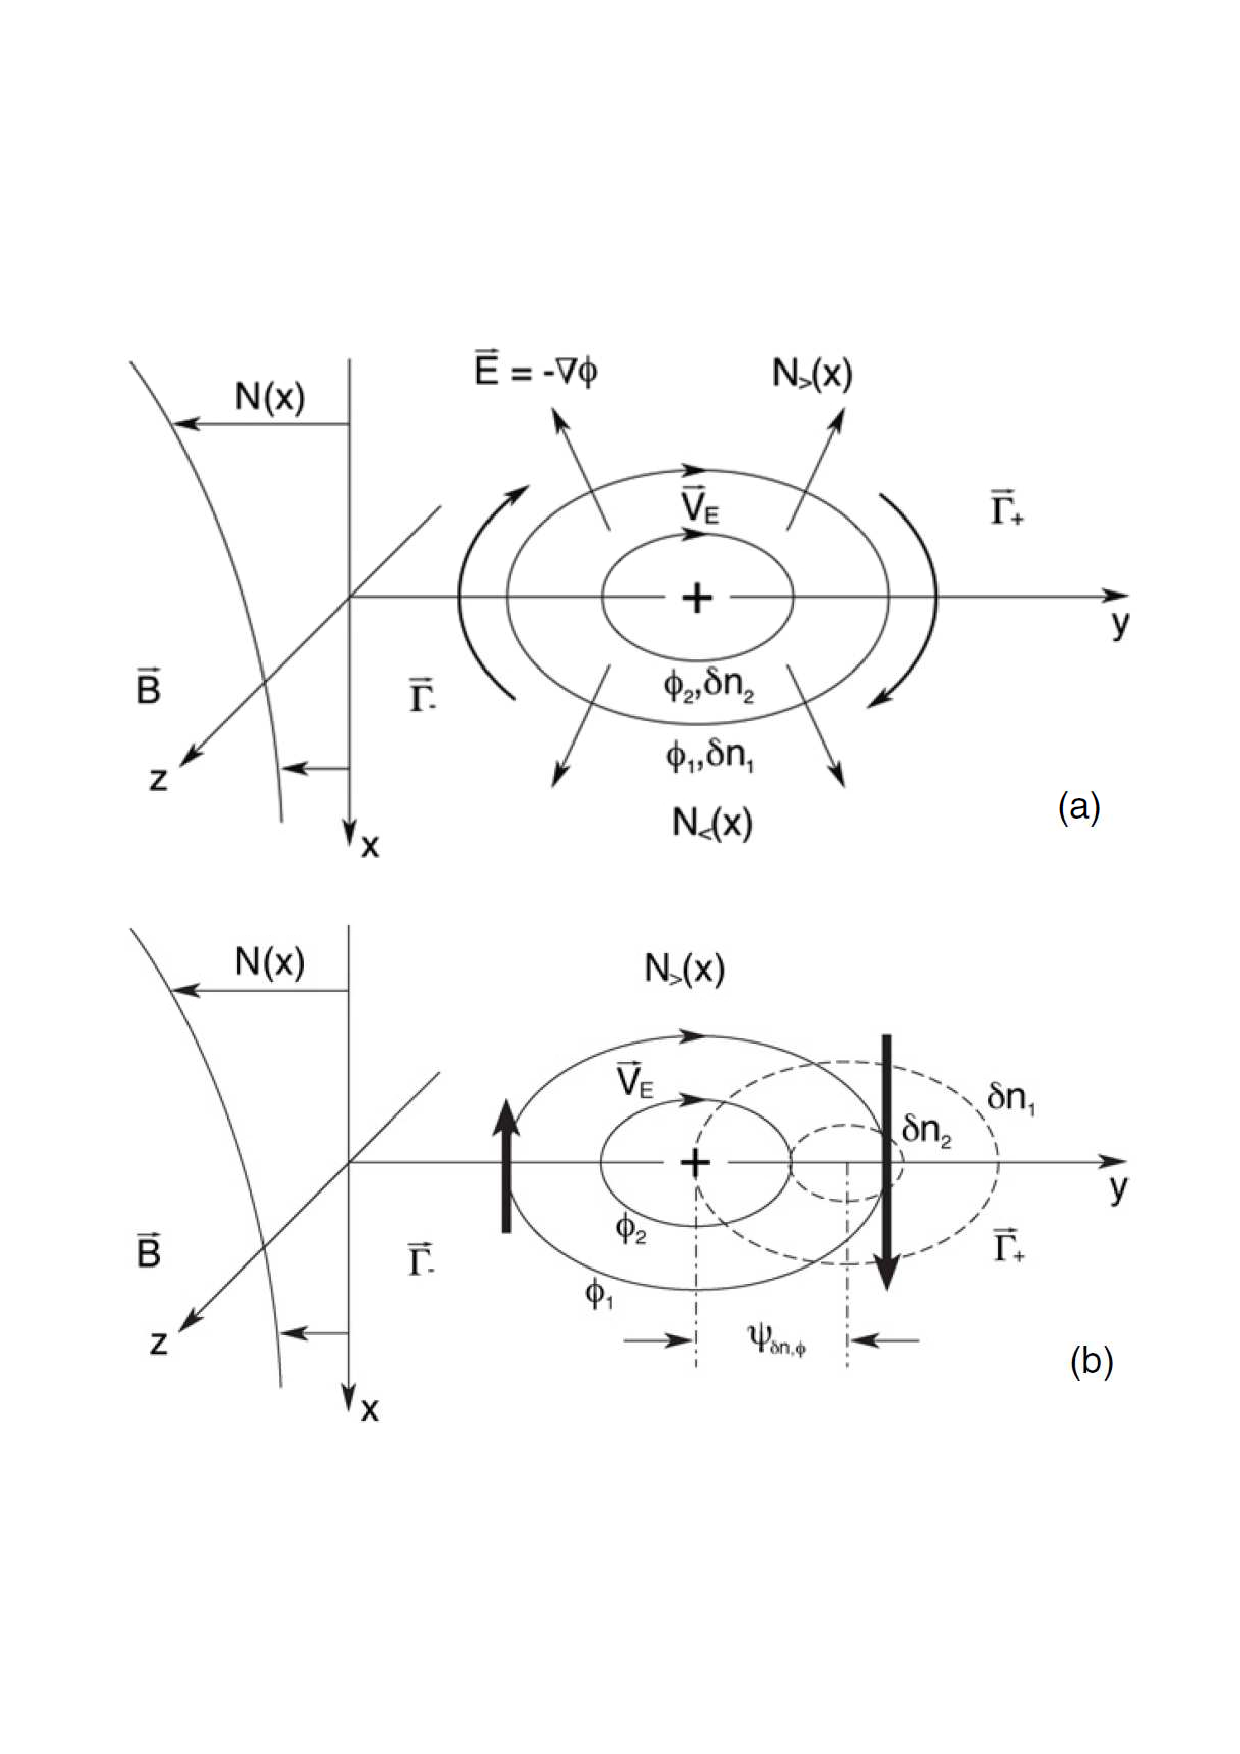
\includegraphics[scale=.5]{figures/turbulencefigure}
  \caption*{\small (a) Fluctuations without parallel electron dissipation. (b) Fluctuations with finite electron dissipation. Figure from Tynan et al 2009. Copyright 1999 by the American Physical Society.}
\end{figure}

\subsection{General Drift Turbulence Characteristics}

Perpendicular drift wave turbulence is characterized by $\rho_{S}$, with $k_{||} \ll k_{\bot}$ and $k_{\bot}\rho_{S}$ depending on dissipative mechanism, linear free energy source, and nonlinear energy transfer.\\

\index{Ion thermal gradient instability}

\noindent Ion thermal gradient (ITG) turbulence occurs when $\eta_{i} > \eta_{\textrm{crit}} \sim 1$ and has the following approximate characteristics \cite{tynan}
\fla{k_{\bot} \rho_{s} &\sim 0.1-0.5 &}
\fla{R/L_{T_{i}} &> R/L_{T_{i}}|_{\textrm{crit}} \sim 3-5 &}
\fla{v_{ph} &\sim v_{di} &}

\index{Trapped electron mode}
\index{Electron thermal gradient instability} 
\noindent Trapped electron mode (TEM) instabilities occurs at approximately $k_{\bot}\rho_{S} \sim 1$. At higher wavenumbers the TEM transitions into the electron thermal gradient (ETG) instability with $\eta_{e} > \eta_{\textrm{crit}} \sim 1$ and the following approximate characteristics \cite{tynan}
\fla{k_{\bot} \rho_{s} &\sim 1-10 &}
\fla{R/L_{T_{e}} &> R/L_{T_{e}}|_{\textrm{crit}} \sim 3-5 &}

\index{Passing particle modes}
\subsection{Passing Particle Instabilities}
In this section, it is assumed that $k_{||} v_{te}>> \omega >> k_{||}v_{ti}$, such that electrons respond to the electrostatic potential. Also, the frequency of the magnetic curvature drifts is assumed to be \scite{wesson}{422}
\fla{\omega_{di} &= 2 L_{n}\omega_{*i}/R \ll \omega &}

\index{Passing particle dispersion relation}
\noindent
The passing particle dispersion relation \scite{wesson}{424}
\fla{ \left[\rho_{i}^{2} \frac{\partial^{2}}{\partial x^{2}} - 
  \left(\frac{L_{n}/R}{b^{1/2} (T_{e}/T_{i}) q \Omega} \right)^{2}\left( \frac{\partial}{\partial \theta} + i k_{\theta} s x \right) - 
  \frac{2 R/L_{n}}{(T_{e}/T_{i}) \Omega} \left(\cos\theta +  \frac{i \sin\theta}{k_{\theta}} \frac{\partial}{\partial x} \right)\right. -&\\
  \left.\left(\frac{\Omega-1}{(T_e/T_i) \Omega + (1+\eta_i)} + b \right)\right] \tilde{\phi} &= 0 &}
\hangindent=0.25in where x is the distance from the reference mode rational surface $\textrm{m}=\textrm{n} q(\textrm{r})$ and $\tilde{\phi}$ is the perturbed electrostatic potential.\\

\index{Ion thermal gradient instability}
\index{ITG |see{Ion thermal gradient instability}}
\noindent
Ion thermal gradient (ITG, eta-i, $\eta_i$) toroidal frequency \scite{wesson}{428}
\fla{ \omega_\mathrm{ITG} &\approx (\eta_{i} \omega_{*i}\omega_{di})^{1/2} &}

\noindent
ITG critical instability limit \scite{wesson}{429}
\fla{ \eta_{ic} &= \left\{
\begin{gathered}
   1.2 \hspace{1cm}\hfill R/L_{n} < (R/L_{n})_{\textrm{crit}} \\
   \frac{4}{3} \left(1 + \frac{T_{i}}{T_{e}} \right) \left( 1 + 2s/q \right) R/L_{n}\hspace{1cm}\hfill  R/L_n > (R/L_n)_\mathrm{crit} \\
\end{gathered} \right. &}

\indent where
\fla{(R/L_{n})_{\textrm{crit}} &= \frac{0.9}{(1+T_{i}/T_{e})(1+2s/q)} &}


% ?????
% If $R/L_{n} < (R/L_{n})_{crit}$ then $\eta_{ic} = 1.2$

\index{Electron thermal gradient instability} 
\index{ETG|see{Electron thermal gradient instability}}
\noindent
Electron thermal gradient (ETG, $\eta_{e}$ mode) dispersion relation with $T_{i}\approx T_{e}$ \scite{wesson}{429}
\fla{-\frac{k_{||}^{2} v_{te}^{2}}{\omega^{2}} \left( 1- \frac{\omega_{*e}}{\omega} (1 + \eta_{e}) \right)+1 + \frac{\omega_{*e}}{\omega} &= 0 &} 

\indent If $\eta_{e} \gg 1$ then there is an unstable mode with \scite{wesson}{429}
$\omega \approx (-k_{||}^{2}v_{te}^{2} \eta_{e} \omega_{*e})^{1/3}$

\index{Trapped particle modes}
\subsection{Trapped Particle Modes}

\index{Trapped particle dispersion relation}
The collisionless trapped particle dispersion relation \scite{wesson}{432}
\fla{\frac{1}{\sqrt{2 \epsilon}} \left( \frac{1}{T_{i}} + \frac{1}{T_{e}} \right) &= \frac{1}{T_{i}} \frac{\omega-\omega_{*i}}{\omega-\bar{\omega}_{di}} + \frac{1}{T_{e}} \frac{\omega-\omega_{*e}}{\omega-\bar{\omega}_{de}} &}

\indent where 
\fla{\bar{\omega}_{dj} &= \frac{\omega_{dj}}{2} \left[ \left(\frac{v_{||}}{v_{Thj}} \right)^{2} + \left( \frac{v_{\bot}}{2 v_{Thj}} \right)^{2} \right] \{ \cos \theta + \frac{k_{r}}{k_{\theta}} \sin \theta \} &}

\index{Trapped ion mode}
\noindent This dispersion relation gives rise to the trapped ion mode if $\nu_{\textrm{eff}}=\nu_{j}/\epsilon > \omega_{dj}$ and has growth/frequency\scite{wesson}{433-434}
\fla{\omega &= \frac{\sqrt{2 \epsilon}}{1 + T_{e}/T_{i}} \omega_{*e} - i \frac{\nu_{i}}{\epsilon} + i \frac{\epsilon^2}{(1+T_{e}/T_{i})^2} \frac{\omega_{*e}^{2}}{\nu_{e}} &}

This mode has the largest imaginary part if $\nu_{e}\approx \epsilon^{3/2} \omega_{*e}$.\\

\index{Trapped electron mode}
\index{TEM|see{Trapped electron mode}}
\noindent
The TEM can be calculated due to the trapped particle dispersion
relation. The mode is driven by trapped electron collisions and
electron temperature gradients. \scite{wesson}{434-435}\\

\noindent If $\nu_{\textrm{eff}} \gg \omega_{*e}$ then the growth rate is 

\fla{\gamma &\approx \epsilon^{3/2} \frac{\omega_{*e}^{2}}{\nu_{e}} \eta_{e} &}

\begin{table}
  \centering
  \begin{tabular}{c c c c}
    \hline
    Parameter\T&  Approximate range          &  Approximate length &  Mode\\
             \B&  in $k_\theta$ (cm$^{-1}$) &  scale(cm)          & \\
    \hline\hline
    \multirow{5}{*}{Density fluctuations ($\tilde{n}$)}\T& $<$ 1              & 60       & ITG \\
                                  & $<$ 2              & 1        & ITG, TEM \\
                                  & $<$ 7              & 1-10     & ITG, TEM \\
                                  & 3-12 & 1        & TEM \\
                                  & $>$ 20             & 1, 20    & ETG \\
    Temperature fluctuations ($\tilde{T_e}$)                 & $<$ 1              & 1        & ITG \\
    Flows, GAMs, ZF               & $<$ 1              & 1        & ITG \\
    $\tilde{n_e}\tilde{T_e}$ cross phase    \B& $<$ 1              & 1        & ITG\\
    \hline
  \end{tabular}
\end{table}
